\documentclass[arhiv]{izpit}
\usepackage{times}
\usepackage{fouriernc}
\usepackage{tikz}
\renewcommand{\ttdefault}{txtt}

\begin{document}

\izpit{Programiranje I: 1.\ kolokvij}{10.\ december 2012}{
  Čas reševanja je 100 minut.
  Doseženih 100 točk šteje za maksimalno oceno.
  Veliko uspeha!
}

%%%%%%%%%%%%%%%%%%%%%%%%%%%%%%%%%%%%%%%%%%%%%%%%%%%%%%%%%%%%%%%%%%%%%%
\naloga[25 točk]

Matrika $A$ je ortogonalna, kadar velja $A^T A = A A^T = I$.
Sestavite funkcijo \verb|naloga1(m)|, ki vrne
  \verb|True|, če seznam seznamov \verb|m| predstavlja ortogonalno matriko, in
  \verb|False|, če je ne.


%%%%%%%%%%%%%%%%%%%%%%%%%%%%%%%%%%%%%%%%%%%%%%%%%%%%%%%%%%%%%%%%%%%%%%
\naloga[25 točk]

\podnaloga[10 točk]
  Razredu \verb|IskalnoDrevo| dodajte metodo \verb|naloga2a(self)|,
  ki izračuna najmanjši element v danem drevesu.
  Metoda naj deluje v času $O(k)$, kjer je $k$ višina drevesa.

\podnaloga[15 točk]
  Razredu \verb|IskalnoDrevo| dodajte metodo \verb|naloga2b(self)|, ki vrne število v drevesu, ki se po absolutni vrednosti najmanj razlikuje od vsebine korena, a mu ni enako. Če takega elementa ni, naj metoda vrne \verb|None|, če pa sta taka elementa dva, naj vrne par obeh. Metoda naj deluje v času $O(k)$, kjer je $k$ višina drevesa.

%%%%%%%%%%%%%%%%%%%%%%%%%%%%%%%%%%%%%%%%%%%%%%%%%%%%%%%%%%%%%%%%%%%%%%
\naloga[25 točk]

Sestavite funkcijo \verb|naloga3(t)|,
ki v času $O(\log n)$ poišče najmanjši element tabele
\[
  \mathtt{t} = [t_1, t_2, \dots, t_n].
\]
Pri tem lahko privzamete, da so vsi elementi $t_i$ med seboj različni
in da ima tabela natanko en lokalni minimum.
Indeks $i$ je lokalni minimum, če velja bodisi
  $t_i < t_{i - 1}$ in $t_i < t_{i + 1}$
  bodisi $i = 1$ in $t_1 < t_2$
  bodisi $i = n$ in $t_n < t_{n - 1}$.

%%%%%%%%%%%%%%%%%%%%%%%%%%%%%%%%%%%%%%%%%%%%%%%%%%%%%%%%%%%%%%%%%%%%%%
\naloga[25+ točk]

Edina stvar,
ki jo mesar Štefan počne raje od izdelovanja pleskavic,
je njihovo urejanje od največje do najmanjše.
Zaradi higienskih standardov
pa Štefan pleskavic ne more kar prijeti v roko,
temveč jih mora obračati z lopatko (oziroma po domače ``špohtlom'') tako,
da lopatko vstavi nekam na sredino in
z njo na glavo obrne kup pleskavic nad njo.

\[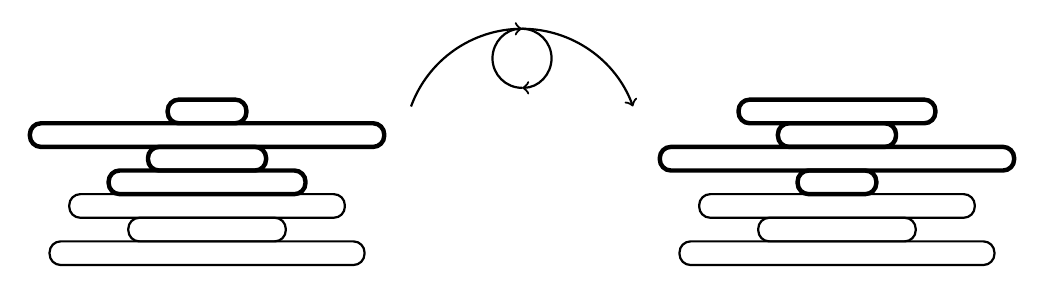
\begin{tikzpicture}[rounded corners, xscale = 0.5, thick]
  \begin{scope}[xshift = -8cm, yscale = 0.3]
    \draw[ultra thick] (-1, 6) rectangle (1, 7);
    \draw[ultra thick] (-4.5, 5) rectangle (4.5, 6);
    \draw[ultra thick] (-1.5, 4) rectangle (1.5, 5);
    \draw[ultra thick] (-2.5, 3) rectangle (2.5, 4);
    \draw (-3.5, 2) rectangle (3.5, 3);
    \draw (-2, 1) rectangle (2, 2);
    \draw (-4, 0) rectangle (4, 1);    
  \end{scope}
  \begin{scope}[yshift = 1.5cm, yscale = 0.5]
    \draw (0, 3) arc (90:160:3cm);
    \draw[->] (0, 3) arc (90:-90:0.75cm);
    \draw[<-] (0, 3) arc (90:270:0.75cm);
    \draw[->] (0, 3) arc (90:20:3cm);
    \end{scope}
  \begin{scope}[xshift = 8cm, yscale = 0.3]
    \draw[ultra thick] (-2.5, 6) rectangle (2.5, 7);
    \draw[ultra thick] (-1.5, 5) rectangle (1.5, 6);
    \draw[ultra thick] (-4.5, 4) rectangle (4.5, 5);
    \draw[ultra thick] (-1, 3) rectangle (1, 4);
    \draw (-3.5, 2) rectangle (3.5, 3);
    \draw (-2, 1) rectangle (2, 2);
    \draw (-4, 0) rectangle (4, 1);    
  \end{scope}
\end{tikzpicture}\]

Če velikosti pleskavic predstavimo s tabelo $[p_1, \dots, p_n]$,
lahko Štefan lopatko vstavi pod $k$. pleskavico, in s tem preuredi tabelo
\[
  [p_1, p_2, \dots, p_{k - 1}, p_k, p_{k + 1}, \dots, p_{n - 1}, p_n]
  \qquad\text{v}\qquad
  [p_1, p_2, \dots, p_{k - 1}, p_n, p_{n - 1}, \dots, p_{k + 1}, p_k].
\]

\podnaloga[5 točk]
  Sestavite funkcijo \verb|naloga4a(t, k)|,
  ki vrne tabelo, ki jo dobimo s tem,
  da v tabeli \verb|t| na glavo obrne podtabelo elementov od \verb|k|. naprej.

\podnaloga[20+ točk]
  Sestavite funkcijo \verb|naloga4b(t)|,
  ki vrne seznam indeksov, nad katerimi moramo obračati elemente tabele,
  da bo na koncu tabela urejena.



\end{document}

